% 角动量定理 角动量守恒

\pentry{角动量定理\ 角动量守恒(单个质点)\upref{AMLaw1}, 牛顿第三定律\upref{New3}}

\textbf{角动量定理}可以表示为
\begin{equation}\label{AMLaw_eq1}
\dv{\vec L}{t} = \vec M
\end{equation}
即系统的角动量对时间的变化率等于所受外力的合力矩.系统可以包括任意选定的若干物体.

\subsection{推导}
推导可类比动量定理\upref{PLaw}.我们已经知道单个质点的角动量,而任何物体都可以划分成若干足够小的微元,每个微元可以看成一个质点.令第 $i$ 个质点的角动量为 $\vec L_i$,力矩为 $\vec M_i$,单个质点的角动量定理\upref{AMLaw1} 为
\begin{equation}
\dv{\vec L_i}{t} = \vec M_i = \vec M_i^{in} + \vec M_i^{out}
\end{equation}
其中 $\vec M_i^{in}$ 和 $\vec M_i^{out}$ 为质点 $i$ 受到的系统内其他质点的力矩和来自系统外的力矩.将该式对所有 $i$ 求和,得到总角动量 $\vec L$ 变化率
\begin{equation}
\dv{\vec L}{t} =\sum_i\dv{\vec L_i}{t} = \sum_i\vec M_i^{in} + \sum_i\vec M_i^{out}
\end{equation}
现在我们只需证明质点系的合内力矩为零即可
\begin{equation}
\sum_i\vec M_i^{in} = \sum_i \vec r_i\cross\sum_j^{j\ne i}\vec F_{j\to i} = \sum_{i,j}^{i\ne j} \vec r_i\cross\vec F_{j\to i}
\end{equation}
其中 $\vec F_{j\to i}$ 是质点 $j$ 对质点 $i$ 的力.现在只考虑任意两个质点 $k$ 和 $l$,在求和中的贡献为
\begin{equation}
\vec r_k\cross\vec F_{l\to k} + \vec r_l\cross\vec F_{k\to l} \equiv \vec M_{l\to k}+ \vec M_{k\to l}
\end{equation}
即 $k$ 对 $l$ 的力矩加 $l$ 对 $k$ 的力矩(两质点的和内力矩).所以若能证明任意两质点的和内力矩为零,则质点系的合内力矩为零.

我们先来看几何证明.如\autoref{AMLaw_fig1}, 根据定义, 力矩的大小等于力力的模长乘以力臂的长度\upref{Torque}, 而一对相互作用力的大小相同, 又由于二者共线, 力臂也重合, 所以两个力矩大小相等. 但是两个力矩的方向一个是顺时针(指向纸内), 一个是逆时针(指向纸外), 所以两力矩互相抵消, 相加为零.

\begin{figure}[ht]
\centering
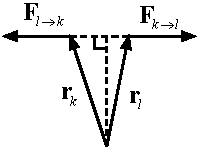
\includegraphics[width=3.7cm]{./figures/AMLaw.pdf}
\caption{两质点的相互作用力对总力矩贡献为零}\label{AMLaw_fig1}
\end{figure}

再在看代数的方法:我们先沿着两质点的连线写出相互作用力 $\vec F_{l\to k} = \alpha(\vec r_k - \vec r_l)$, $\vec F_{k\to l} = \alpha(\vec r_l - \vec r_k)$,直接计算总角动量得
\begin{equation}
\vec r_k\cross\vec \alpha(\vec r_k - \vec r_l) + \vec r_l\cross\alpha(\vec r_l - \vec r_k) = 0
\end{equation}

